\documentclass[usenames,dvipsnames, 10pt]{beamer}
\usepackage[utf8]{inputenc}
\usepackage{verbatim}
\usepackage{subfigure}
\usepackage{graphicx}
\usepackage{caption}
\usepackage{array}
\setlength{\extrarowheight}{2pt} % Увеличение отступа на 2pt
%\setbeamertemplate{caption}[numbered]

\usepackage[english,russian]{babel}
\usetheme{MMF}

\newtranslation[to=russian]{Theorem}{Теорема}
\newtranslation[to=russian]{Example}{Пример}
\newtranslation[to=russian]{Corollary}{Следствие}
\newtranslation[to=russian]{Lemma}{Лемма}
\newtranslation[to=russian]{Abstract}{Abstract}
\renewcommand\proofname{Proof}
%\renewcommand{abstract}{Abstract}
%%% Bibliography
\usepackage[style=authoryear,backend=biber]{biblatex}
\addbibresource{bibliography.bib}

\DeclareNameAlias{author}{first-last}

\usepackage{silence}
\WarningFilter{biblatex}{Patching footnotes failed}

\newcommand{\pdfnewline}{\texorpdfstring{\newline}{ }} 
\newcommand{\framefill}{\vskip0pt plus 1filll}

\title[]{Классификация изображений бинарными нейронными сетями с расширенной информацией}
\date[May 2023]{}
\author[Антон Чанчиков]{
  Чанчиков Антон Юрьевич. Бакалавриат, 4 курс, группа 19122 \newline \newline
  Научные руководители:
  \begin{itemize}
      \item   Тарков Михаил Сергеевич. Профессор кафедры Вычислительных систем ММФ НГУ,  к.т.н., доцент
      \item   Городничев Максим Александрович. Старший преподаватель кафедры Вычислительных систем ММФ НГУ
  \end{itemize}
  \pdfnewline
}
\institute{Department of Mathematics and Mechanics, 

Novosibirsk State University}

\begin{document}

\begin{frame}
\titlepage
\end{frame}

\begin{frame}{Содержание}
\tableofcontents
\end{frame}

\section{Введение}
\begin{frame}
\frametitle{\phatom}
\centering
\Large \textbf{Введение}
\end{frame}


\begin{frame}
\frametitle{Сверточные нейронные сети}
\begin{figure}[h!]
\center{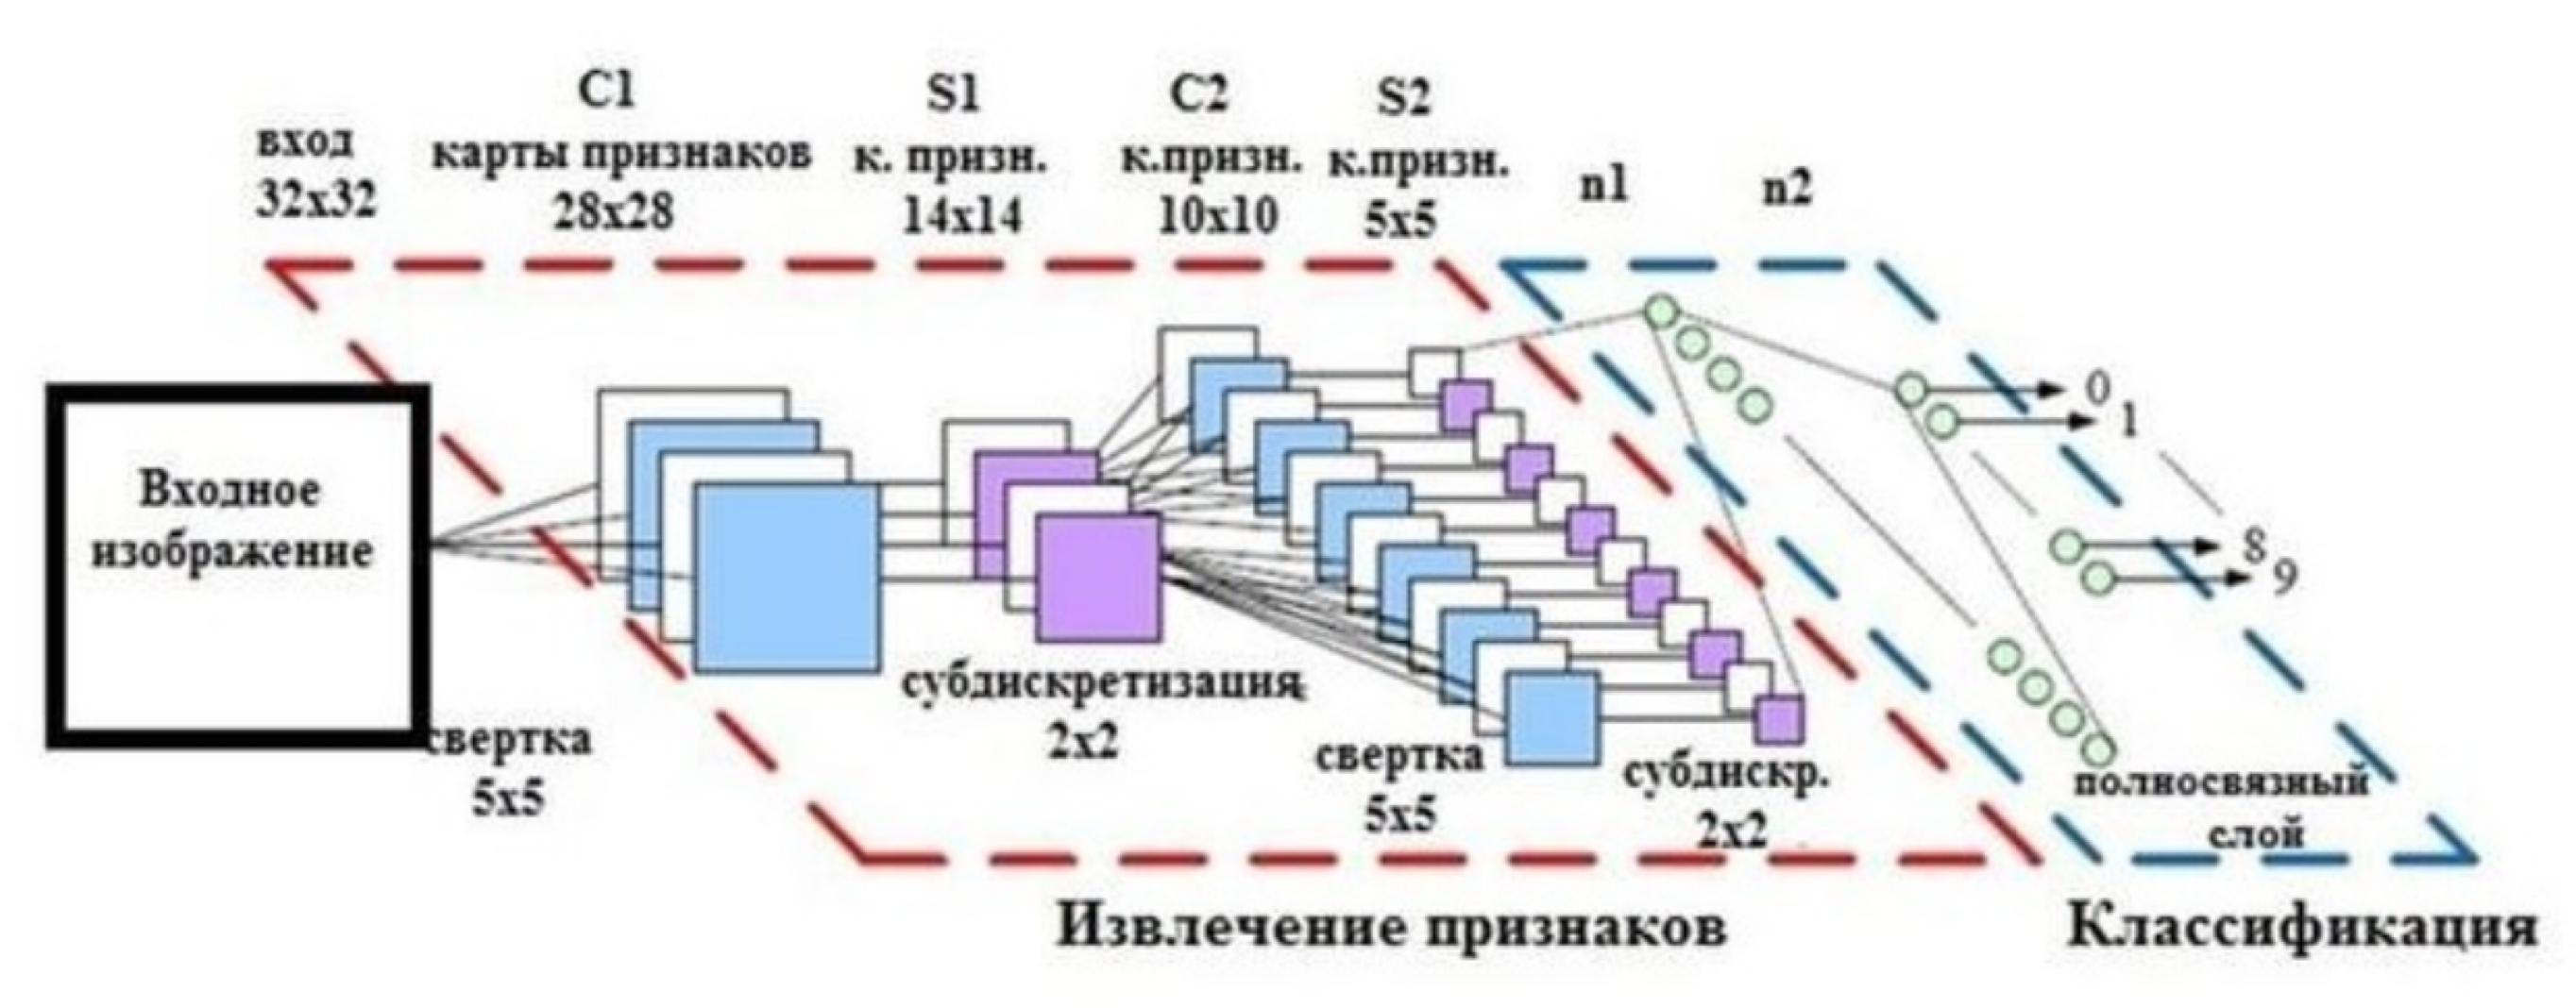
\includegraphics[width=0.9\linewidth]{graphics/CNN.png}}
\label{image:CNN}
\end{figure}
\end{frame}

\begin{frame}
\frametitle{Задача классификации изображений}

Постановка задачи: определить, к какому классу наиболее вероятно принадлежит входное изображение.

\begin{figure}[h!]

\subfigure[CIFAR-10. Трехканальные цветные изображения, разрешение 32х32]{
  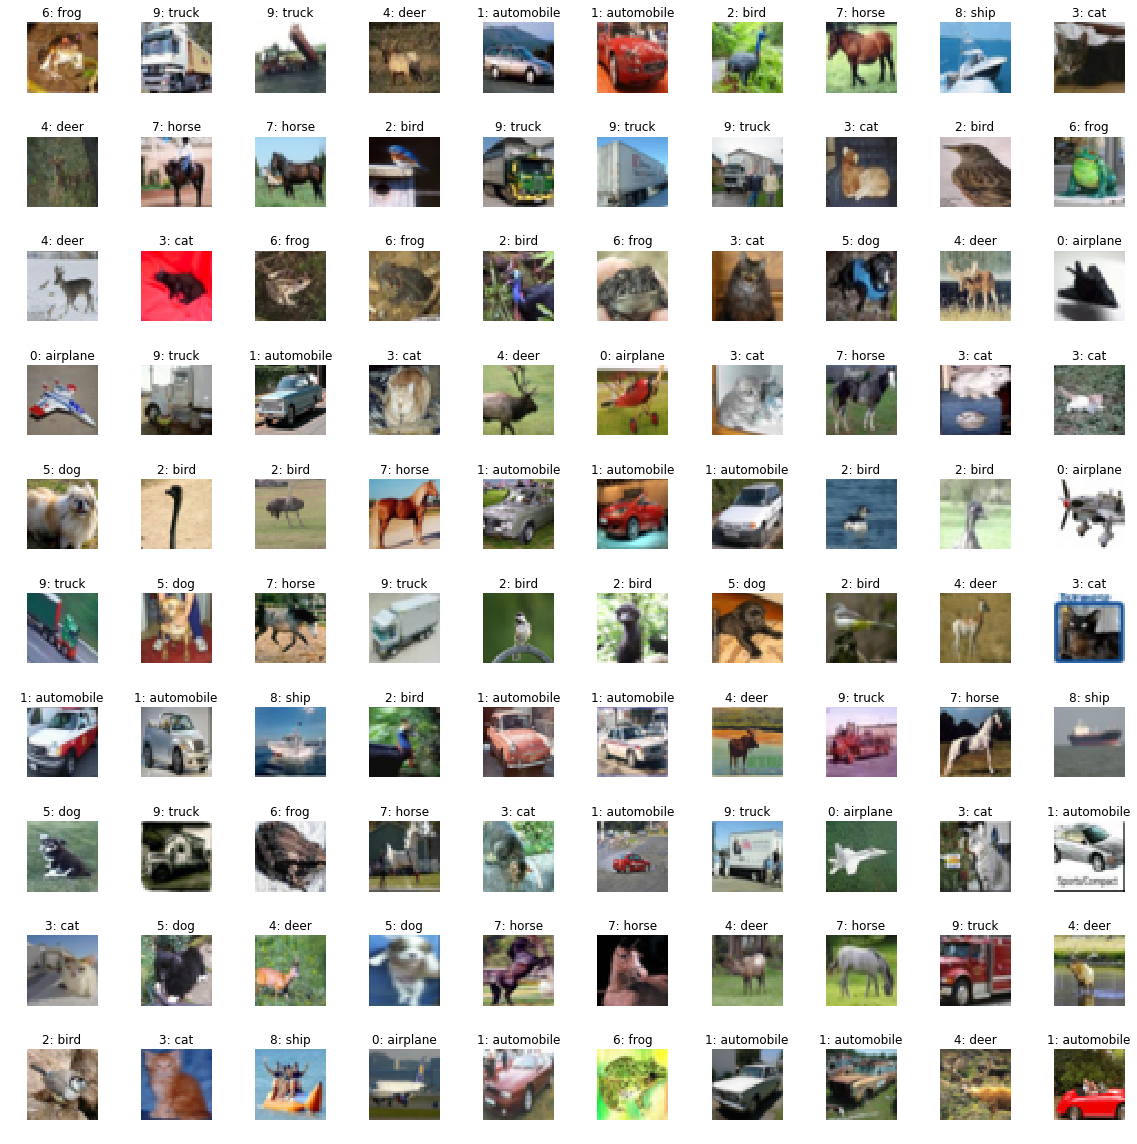
\includegraphics[width=0.4\linewidth]{graphics/CIFAR10.png}
  \label{image:CIFAR}
}
%\caption{Comparison of MNIST and CIFAR-10}
\end{figure}

\end{frame}

\begin{frame}
\frametitle{Бинарные нейронные сети}
\vskip 0.5cm
Идея: \begin{equation*}\label{2.1}
\small
b_w = \text{sign}(w) =
    \begin{cases}
    \begin{aligned}
        +1 & \text{, если } w \geq 0 \\
        -1 & \text{, иначе }
    \end{aligned}
    \end{cases}
    , \quad b_x = \text{sign}(x) = 
    \begin{cases}
    \begin{aligned}
        +1 & \text{, если } x \geq 0 \\
        -1 & \text{, иначе }
    \end{aligned}
    \end{cases}
\end{equation*}
\begin{flushright}
где $w$ и $x$ - веса и активации полноточной нейронной сети,\\
$b_w$ и $b_x$ - бинарной нейронной сети.
\end{flushright}


Тогда выход сети представляет из себя побитово примененные операции XNOR и POPCOUNT к множествам $B_w$ и $B_x$
\begin{equation*}
    Y = (B_w \oplus B_x) \cdot  \alpha
\end{equation*}
\end{frame}

\begin{frame}
\frametitle{Бинарные нейронные сети}
  \begin{columns}
    \column{0.5\textwidth} % Ширина первой колонки
    \begin{center}
      \textbf{Преимущества}
    \end{center}
    \vspace{0.2cm} % Промежуток между заголовком и содержимым колонки

    \begin{center}
      \begin{itemize}
          \item Уменьшение нагрзуки на вычисления
          \item Снижение веса модели
      \end{itemize}
    \end{center}

    \column{0.5\textwidth} % Ширина второй колонки
    \begin{center}
      \textbf{Недостатки}
    \end{center}
    \vspace{0.2cm} % Промежуток между заголовком и содержимым колонки

    \begin{center}
        \begin{itemize}
          \item Большие потери информации при бинаризации
        \end{itemize}
    \end{center}
  \end{columns}


\end{frame}

\section{Цель и задачи}
\begin{frame}
\frametitle{\phatom}
\centering
\Large \textbf{Цель и задачи}
\end{frame}

\begin{frame}
\frametitle{Цель и задачи}
Цель - разработка и сравнительное исследование методов оптимизации бинарных нейронных сетей с расширенной информацией.
\vskip 0.5cm
Для достижения указанной цели были поставлены следующие задачи:
\begin{itemize}
    \item Выбрать архитектуры сверточных нейронных сетей для классификации изображений.
    \item Провести их бинаризацию и улучшение.
    \item Оценить качество, время работы и количество выполняемых операций в процессе классификации изображений новыми бинарными сетями.
    \item Cравнить полученные результаты для разных сверточных сетей.
\end{itemize}
\end{frame}


\section{Обзор}
\begin{frame}
\frametitle{\phatom}
\centering
\Large \textbf{Обзор}
\end{frame}
\begin{frame}
\frametitle{Связанные работы}
С 2016 по сентябрь 2022 г. - не менее 239 фундаментальных разработок в теме бинарных нейронных сетей.

\vskip 0.5cm


\begin{itemize}
	\item ReActNet предлагает для бинаризации использовать функции с            обучаемыми порогами по входным каналам, что позволяет подавать на вход сети подавать больше различной информации для анализа.
             \begin{equation*}\label{2.2}
                \small
                RSign(x^i) =
                \begin{cases}
                \begin{aligned}
                    +1 \text{, если } x^i \geq \beta^i
                    \\ -1 \text{, если } x^i < \beta^i
                \end{aligned}
                \end{cases}
                % \parbox{10em}{
                %  \math{i = 1, .., I} \\
                % \math{k = 1, .., K}}
            \end{equation*}
	\item IR-Net перед бинаризацией весов предлагает их сбалансировать            и стандартизовать для уменьшения эффекта потери информации.
             \begin{equation*}
                \small
                w_{std} = \frac{\widehat{w}}{\sigma(\widehat{w})}, \ \widehat{w} = w - \bar w
            \end{equation*}
\end{itemize}
\end{frame}


\begin{frame}
\frametitle{БНС с улучшенной информацией}
\begin{itemize}
	\item Использование K функций RSign
                \begin{equation*}
                    b_x^{i,k} = RSign^{k}(x^{i}) =
                    \begin{cases}
                    \begin{aligned}
                        +1 \text{, если } x^{i} \geq \beta^{i,k}
                        \\ -1 \text{, если } x^{i} < \beta^{i,k}
                    \end{aligned}
                    \end{cases}
                    % \parbox{10em}{
                    %  \math{i = 1, .., I} \\
                    % \math{k = 1, .., K}}
                \end{equation*}
        \item Для обработки пакетов вводится обобщенная двочиная свертка
                \begin{equation*}
                Y^k = BConv (B_w, B_x^k) = (B_w \oplus B_x^k) \cdot  \alpha
                \end{equation*}
	\item Стандартизация весов, как в IR-Net, и использование особой           функции IEE для бинаризации весов. Особенность в том, что она             постепенно в процессе обучения аппроксимирует функцию знака,           придавая градиентам весов ненулевые значения
            \vskip 0.2cm
            \begin{figure}[h!]
            \center{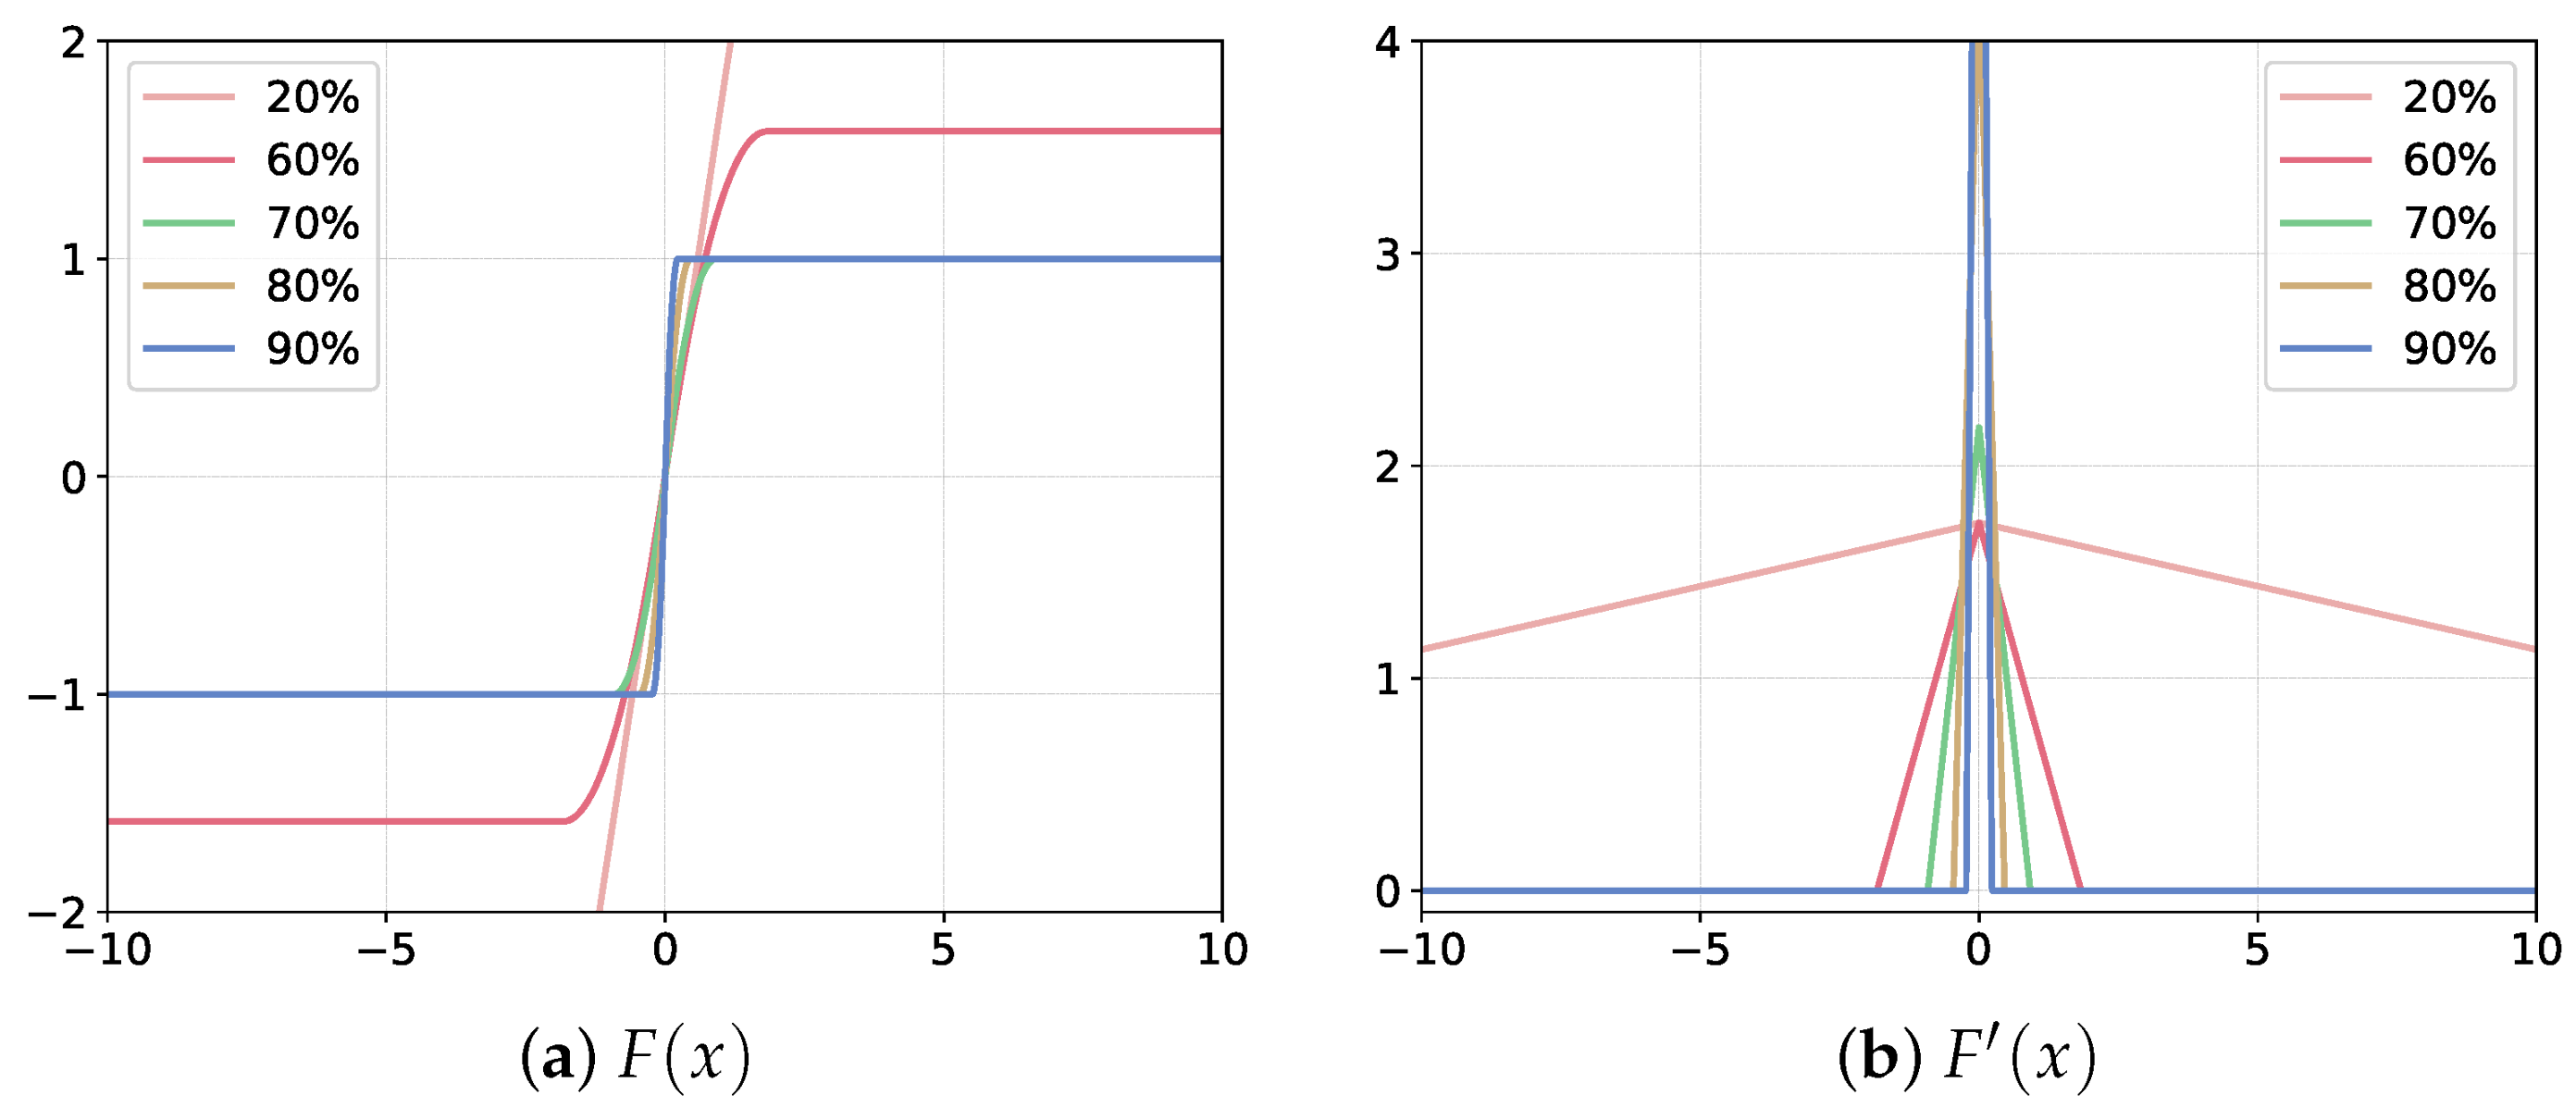
\includegraphics[width=0.6\linewidth]{graphics/IEE.png}}
            \label{image:IEE}
            \end{figure}
\end{itemize}
\end{frame}

\begin{frame}
\frametitle{БНС с улучшенной информацией}
\begin{figure}
    \center{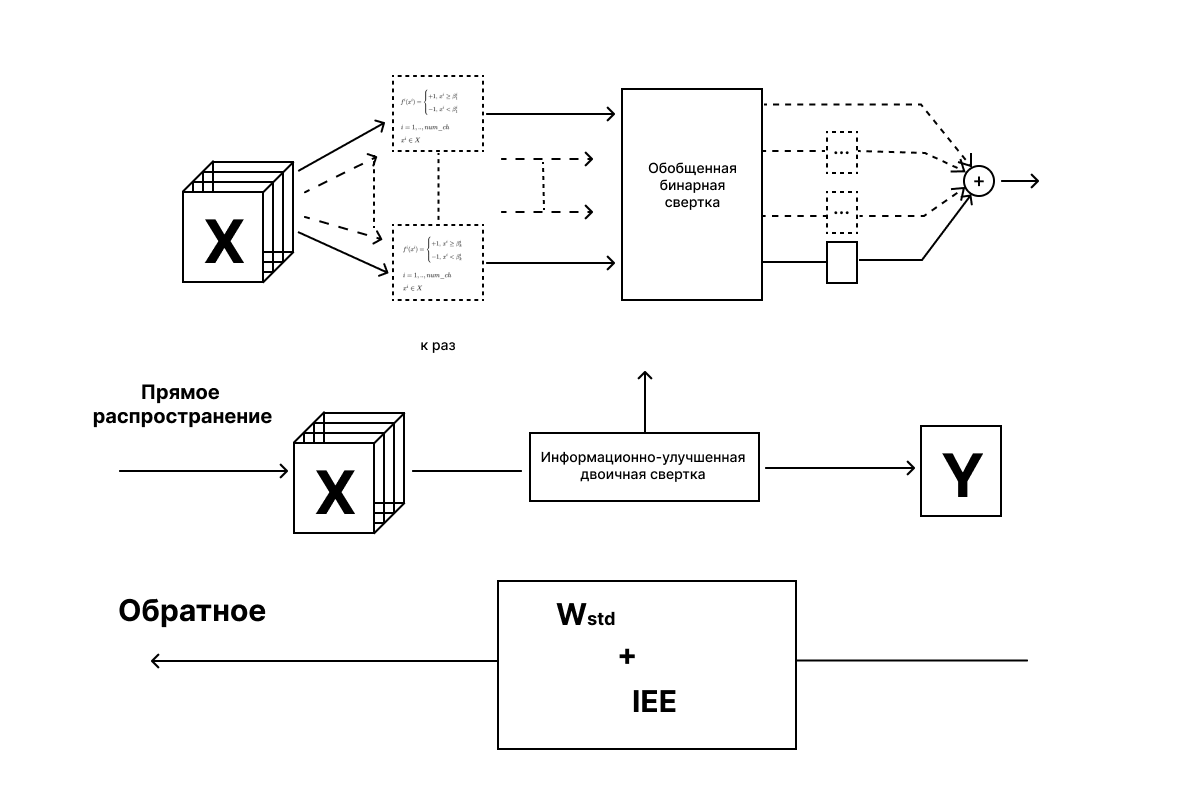
\includegraphics[width=0.9\linewidth]{graphics/IE-Net.png}}
    \caption*{\small\textbf{Структура БНС с улучшенной информацией}}
    \label{image:IE-Net}
\end{figure}
\end{frame}

\section{Исследовательская основа}
\begin{frame}
\frametitle{\phatom}
\centering
\Large \textbf{Исследовательская основа}
\end{frame}

\begin{frame}
\frametitle{Выбранные архитектуры}
  \begin{columns}
    \column{0.5\textwidth} % Ширина первой колонки
    \begin{center}
      \textbf{ResNet}
    \end{center}
    \vspace{0.1cm} % Промежуток между заголовком и содержимым колонки

    \begin{center}
      \begin{itemize}
          \item Высокая точность обработки изобрежний
          \item Требует больших вычислительных мощностей
          \item Глубокая сеть с большим количеством параметров
      \end{itemize}
    \end{center}

    \column{0.5\textwidth} % Ширина второй колонки
    \begin{center}
      \textbf{MobileNetV2}
    \end{center}
    \vspace{0.2cm} % Промежуток между заголовком и содержимым колонки

    \begin{center}
        \begin{itemize}
          \item Высокая точность обработки изобрежний
          \item Эффективное потребление вычислительных ресурсов
          \item Малый вес
        \end{itemize}
    \end{center}
  \end{columns}
\end{frame}

\section{Методы оптимизации}
\begin{frame}
\frametitle{\phatom}
\centering
\Large \textbf{Методы оптимизации}
\end{frame}
\begin{frame}
\frametitle{Методы оптимизации}
\begin{itemize}
    \item Регуляризация - методика ограничения модели для улучшения ее обобщающей способности
    \item Аугментация - расширение исходного набора данных, путем применения к изображению некоторых операций, таких как поворот, сдвиг, инвертация каналов и другие
    \item Дистилляция - тактика обучения небольшой модели используя знания другой, более масштабной сети
    \item Обрезание - удаление незначимых весов сети для облегчения ее веса при небольших потерях точности
\end{itemize}
\end{frame}

\section{Разработка фреймворка}
\begin{frame}
\frametitle{\phatom}
\centering
\Large \textbf{Разработка фреймворка}
\end{frame}
\begin{frame}
\frametitle{Разработка фреймворка}
Для реализации большого количества экспериментов с использованием различных моделей и методов было принято решение создать исследовательский фреймворк для более легкой, гибкой и быстрой работы.
\vskip 0.5cm
Он включает в себя:
\begin{itemize}
    \item Реализацию всех методов, вариантов моделей и других опциональных вещей, описанных ранее
    \item Возможность менять гиперпараметры, модели и наборы данных для исследований
    \item Возможность запускать несколько экспериментов разом из некоторого фиксированного пространства методов для мгновенного сравнения результатов
\end{itemize}
\end{frame}

\section{Эксперименты}
\begin{frame}
\frametitle{\phatom}
\centering
\Large \textbf{Эксперименты}
\end{frame}
\begin{frame}{Результаты ResNet18}
    \vskip -0.4cm
    \centering
    \begin{tabular}{|c|c|c|}
        \hline
        Значение K & Точность & Время обучения с/эпоха (min, max) \\
        \hline
        Небинарная & 0.89 & 25.9; 28.4 \\
        1 & 0.5958 & 37.9; 40.67 \\
        2 & 0.736 & 61.6; 65.1\\
        \textbf{3} & \textbf{0.757} & \textbf{83.2; 90.9}\\
        4 & 0.7292 & 105; 123.7\\
        5 & 0.744 & 104.3; 107.4\\
        6 & 0.737 & 122.2; 128.4\\
        \hline
    \end{tabular}
    \vskip 0.3cm
    \begin{tabular}{|c|c|c|c|}
        \hline
        Тип сети & FLOPS & GPU Memory usage & Вес  \\
        \hline
        Небинарная & $2.7 \cdot 10^9$ & 6.1Gb & 42.26Mb \\
        Бинарная $(K=3)$ & $2.43 \cdot 10^8$ & 4.8Gb & 4.64Mb \\
        \hline
    \end{tabular}
    \vskip 0.3cm
    \begin{tabular}{|c|c|c|c|c|c|c|}
        \hline
        Тип сети & W/o & +WD & +LS & +RA & -LS & +LS+DP \\
        \hline
        Небинарная & 0.89 & 0.8573 & 0.8503 & 0.9201 & 0.9115 & 0.9150 \\
        Бинарная & 0.757 & 0.7737 & 0.7641 & 0.8488 & 0.8566 & 0.8511\\
        \hline
    \end{tabular}
    
\end{frame}

\begin{frame}
\frametitle{Результаты MobileNetV2}
    \centering
    \vskip -0.4cm
    \begin{tabular}{|c|c|c|}
        \hline
        Значение K & Точность & Время обучения с/эпоха (min, max) \\
        \hline
        Небинарная & 0.8211 & 49.53 ; 52.18 \\
        1 & 0.2915 & 85.57; 89.15 \\
        \textbf{2} & \textbf{0.4684} & \textbf{99.76; 105.0} \\
        3 & 0.4571 & 117.36; 124.01\\
        4 & 0.4603 & 141.5; 148.91\\
        5 & 0.4725 & 178.34; 185.28\\
        6 & 0.4518 & 194.57; 199.13\\
        \hline
    \end{tabular}
    \vskip 0.3cm
    \begin{tabular}{|c|c|c|c|}
        \hline
        Тип сети & FLOPS & GPU Memory usage & Вес  \\
        \hline
        Небинарная & $3 \cdot 10^{9}$ & 3.2Gb & 6.53Mb \\
        Бинарная $(K=2)$ & $1.9 \cdot 10^{8}$ & 2.6Gb & 0.87Mb \\
        \hline
    \end{tabular}
    \vskip 0.3cm
    \centering
    \begin{tabular}{|c|c|c|c|c|c|c|}
        \hline
        Модель & W/o & +WD & +LS & +RA & -LS & +LS+DP \\
        \hline
         MobNetV2 & 0.8124 & 0.8289 & 0.8275 & 0.9031 & 0.9043 & 0.905 \\
        \hline
    \end{tabular}
\end{frame}

\begin{frame}{Перенос знаний}
    \centering
    \begin{table}[h]
    \begin{tabular}{|c|c|c|c|c|c|c|}
        \hline
        Модель & W/o & +WD & +LS & +RA & -LS & +LS+DP \\
        \hline
         Бинарная (K=3)& 0.8105 & 0.8356 & 0.8491 & 0.89 & 0.8747 & 0.8944 \\
        \hline
    \end{tabular}
    \caption{\centering Дистилляция знаний полноточной ResNet18 на бинарный аналог}
    \label{tab: Distillation}
    \end{table}
\end{frame}

\begin{frame}{Выводы}
    \begin{itemize}
        \item Сильное расширение информации не всегда способно повысить качество модели, то есть из увеличения гиперпараметра K не следует рост точности.
        \vskip 0.3cm
        \item Показано, что применение методов регуляризации в основном улучшает точность сетей, однако для каждой нужно искать индивидуальный путь их применения.
        \vskip 0.3cm
        \item Для бинарных моделей крайне эффективно работает тактика обучения учитель-ученик, стратегия обучения способствует повышению качества ученика.
        \vskip 0.3cm
        \item Теоретические ожидания не всегда оправдываются на практике, что связано с эффективностью программной реализации.
    \end{itemize}
\end{frame}

\begin{frame}{Заключение}
\vskip -0.5cm
\begin{enumerate}
    \item Разработан план экспериментального исследования с целью повышения точности бинарных нейронных сетей с расширенной информацией, предложены методы оптимизации сетей: поиск оптимального количества информации для расширения, комбинация методов регуляризации, которую нужно подбирать вручную для разных архитектур, перенос знаний, который показал себя перспективно для практического применения.
    \vskip 0.5cm
    \item Разработана схема автоматизации исследования и реализован программный фреймворк для ее выполнения.
    \vskip 0.5cm
    \item Проведены эксперименты по изучению поставленных вопросов и показано, что применение некоторых из предложенных методов позволяет повысить точность модели, например, расширение информации, методы регуляризации и расширение датасета для бинарной ResNet18.
\end{enumerate}
\end{frame}

\begin{frame}
\frametitle{\phatom}
    \centering
    \Large
    Q\&A 
\end{frame}

\end{document}